
%% simple table 
% https://www.youtube.com/watch?v=gpzeV-N7wfk&list=PLNnwglGGYoTtW7o4PHFOSWGevcdFa3v3D&index=6 

%\begin{table}
%  \caption{A stunning table}
%  \label{tbl:excel-table}
%  \includegraphics[width=\linewidth]{excel-table}
%\end{table}

\cleardoublepage

\addcontentsline{toc}{chapter}{\numberline{}5eme chapiter}
\addtocontents{lof}{\textbf{Chapter A5}}

\setcounter{chapter}{5}
\setcounter{section}{0}
\setcounter{figure}{0}

\begin{center}
	\Huge\textbf{5eme chapter}
\end{center}

\section{Introduction}
Dans le chapitre précédent, nous avons présenté en détaille les approches que nous avons proposées pour la résolution du problème de l’arbre dominant (DTP). A ce stade nous allons décrire l’environnement de développement de ces approches. Nous allons ainsi présenter une étude expérimentale effectuée pour comparer les résultats des approches proposées avec d’autres approches développées pour la résolution du DTP. Nous effectuant aussi une comparaison entre notre approche de coopération proposée  avec d’autres travaux liés au problème de l’arbre dominant et nous le clôturons avec une conclusion.


\section{Environnement de travail}

\subsection{Environnement matériel}
Pour les tests nous avons utilisé une machine pour toutes les instances, les caractéristiques de la machine sont données dans la figure 1

\begin{figure}[H]
	\centering
	
\includegraphics[width=16cm,height=7cm]{Chap5/1.png}
	\caption{Caractéristiques de la machine utilisée}
	\label{fig:CMU}
\end{figure}

\subsection{Environnement logiciel}
Nous avons opté pour le langage Java, car il offre une grande flexibilité et facilite l’implémentation qui est due au fait qu’il soit totalement orienté-objet.

\textbf{IDE :}
IntelliJ Idea L’environnement de développement choisit est IntelliJ IDEA, spécialement dédié au développement en utilisant le langage Java. Il est proposé par l’entreprise JetBrains et est caractérisé par sa forte simplicité d’utilisation et les nombreux plugins et extensions qui lui sont dédiées.

\section{Jeux de données utilisées}

Afin de tester notre solveur nous avons opté pour l’utilisation de fichiers benchmark qui vont représenter des instances du problème. Les différentes instances sur lesquelles notre étude s’est portée, sont dérivées à partir des mêmes benchmarks de \cite{sundar2013new}. Une instance est considérée comme un graphe de disques, G = ( V, E ) où chaque disque représente la plage de transmission de chaque nœud. Le poids de chaque arête $e_{uv} \in E $ est défini sous la forme w ( u, v ) = $d_{uv}^2$ , où $d_{uv}$ est la distance euclidienne entre deux nœuds u et v. L’hypothèse est que tous les nœuds sont répartis de manière aléatoire dans une zone de  $500m * 500m $  et la plage de transmission de chaque nœud est de 100, 125, 150m.

\section{Expérimentation}
Pour montrer l'efficacité des approches proposées ne se limitent pas à des graphiques ayant une densité particulière, il est nécessaire de prendre en compte différentes valeurs de la portée de transmission. Les valeurs de la plage de transmission que nous avons considérées conduisent à des instances de DTP réalisables difficiles générées aléatoirement (ceux de la plage 100).

Pour ACO, nous avons utilisé une population de 15 fourmis. Nous avons utilisé $\alpha = 1 \, , \, \beta = 1 \, , \, p = 0.05 \, , \, P_0 = 0.1 $. Toutes les valeurs de phéromone sont initialisées à 0,05.Pour BBO, la taille de la population est de 20 individus pour GA .Quant à l’approche de coopération, nous avons utilisé 0.5 comme probabilité initiale, 0,1 pour la valeur de \( \alpha \).

Pour toutes les instances de test, Nous avons autorisé 100 itérations pour chacune des approches proposées. Nous avons laissé nos approches s’appliquer à autant d’itérations que nécessaire pour une qualité optimale. Donner plus d'itérations à nos approches que celles mentionnées ci-dessus n'aura que peu d'impact sur la qualité de la solution.

Toutes ces valeurs de paramètres sont choisies empiriquement. Ces valeurs de paramètres donnent de bons résultats bien qu'elles ne soient pas optimales pour toutes les instances de test.


\subsection{Étude comparative}
Afin de mener à bien une étude comparative entre nos approches et d’autres travaux effectués pour la résolution du DTP, nous avons gardé approximativement le même nombre d’évaluations de la fonction objectif.
Dans le but d’assurer l’intégrité des résultats, nous avons effectué un total de 20 exécutions pour chacune des instances. Les résultats d’exécutions de nos approches (ACO, BBO, GA et la méthode coopérative) sur les instances citées auparavant, sont illustrés dans le Tableau \ref{tab:1}.

Dans le Tableau  \ref{tab:1}, les lignes correspondent aux différentes instances étudiées, quant aux colonnes, elles représentent, pour chaque approche : la meilleure solution obtenue (colonne BS),

la moyenne de toutes les solutions obtenues au fil des 20 exécutions (colonne AVG), le nombre d’évaluations  (colonne NBV) et la colonne qui représente le temps d’exécution de chaque méta en seconde (colonne sec). 
Notez que les meilleures valeurs sont indiquées en gras dans les tableaux comparatifs.

\begin{table}[H]
	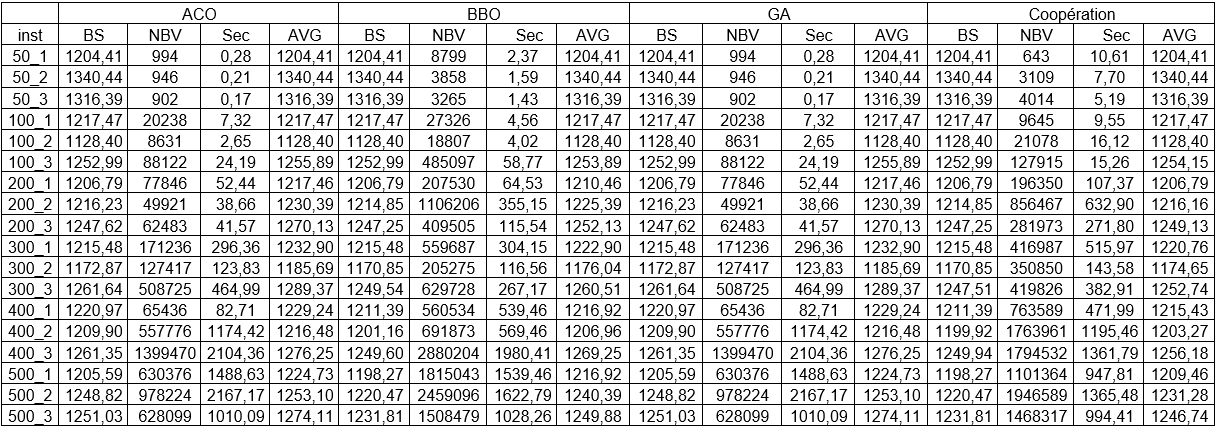
\includegraphics[width=17cm,height=7cm]{Chap5/t1.png}
	\caption{Résultats d’exécutions des  approches proposées}
	\label{tab:1}
\end{table}


\subsubsection{Comparaison de la méthode coopérative avec les autres approches}
Dans ce qui suit nous allons présenter une comparaison entre notre approche coopérative et les autres approches que nous avons développées. Cette comparaison a pour but de montrer l’efficacité de notre approche coopérative par rapport aux approches développées.

\begin{enumerate}[label=\alph*)]
	\item \textbf{Avec l’approche ACO}\\
	D’après le graphe \ref{fig:DEMACOMC} et les résultats présentés dans le tableau \ref{tab:2}, les deux approches sont similaires pour les 11 premiers instances la meilleure solution (BS) obtenue par l’ approche coopérative  est meilleure que celle obtenue par ACO pour les sept  (7) derniers instances. Il faut également noter que la qualité moyenne des solutions (AVG) obtenue par la méthode de coopération est pratiquement meilleure que celle d’ACO pour toutes les instances du problème. Comparé à ACO, le nombre d’évaluation donnée par  l’approche de coopération est relativement faible. Enfin, parlant à propos du temps d’exécutions en général ACO pour ce problème consomme moins de ressources nous trouvons ca normal car ACO n’est  qu’une seule méthode qui s’exécute à la fois contrairement plusieurs méthodes qui se met en compétition.

\begin{table}[H]
	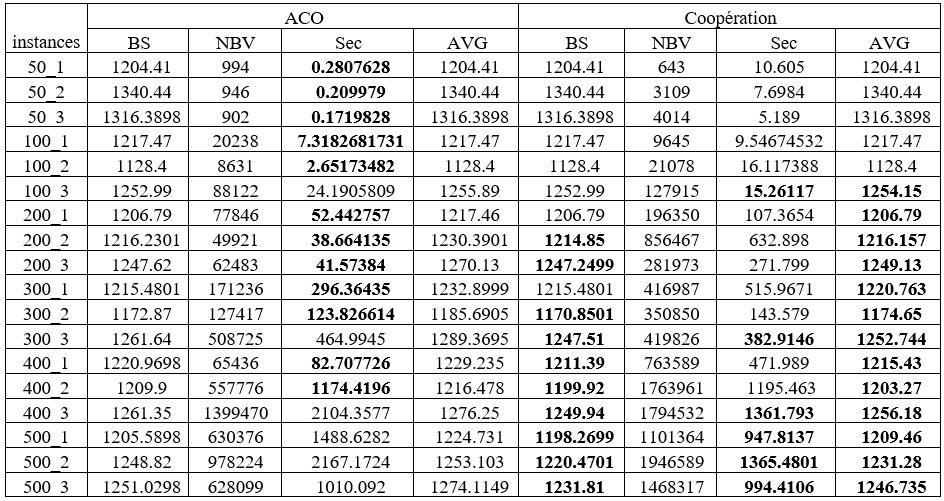
\includegraphics[width=15cm,height=8cm]{Chap5/t2.png}
	\caption{Résultats d’exécutions d’ACO et la méthode de coopération}
	\label{tab:2}
\end{table}

\begin{figure}[H]
	\centering
	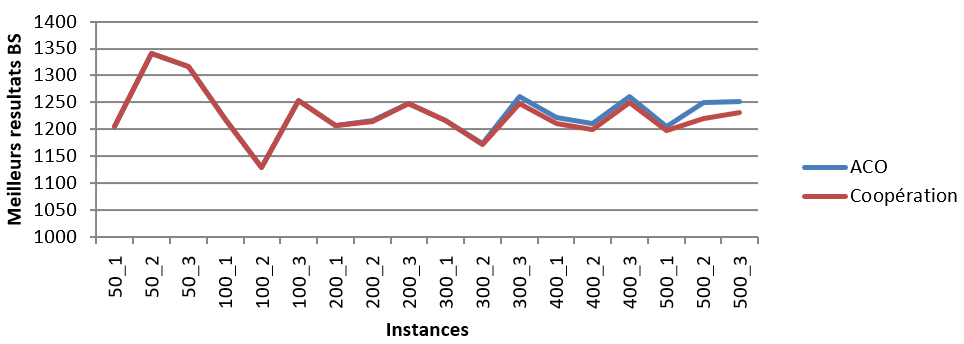
\includegraphics[width=16cm,height=7cm]{Chap5/2.png}
	\caption{Diagrammes d’exécutions de la méthode ACO et la méthode coopérative}
	\label{fig:DEMACOMC}
\end{figure}

	\item \textbf{Avec l’approche BBO}
\begin{table}[H]
	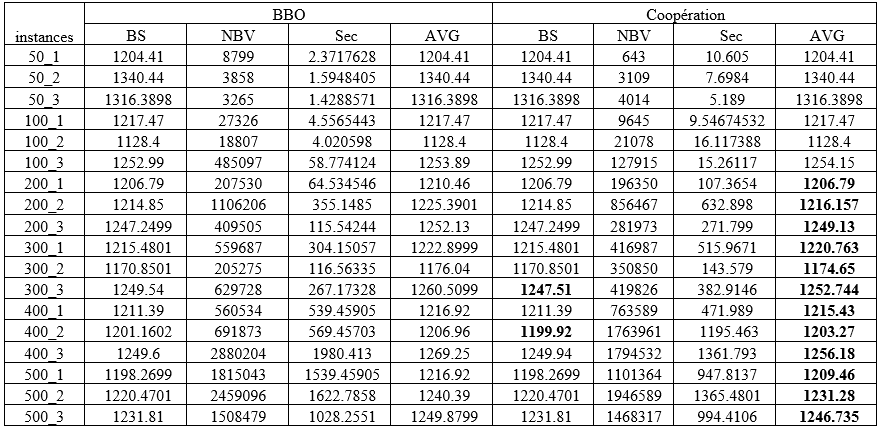
\includegraphics[width=15cm,height=8cm]{Chap5/t3.png}
	\caption{Résultats d’exécutions de BBO et la méthode de coopération}
	\label{tab:3}
\end{table}

\begin{figure}[H]
	\centering
	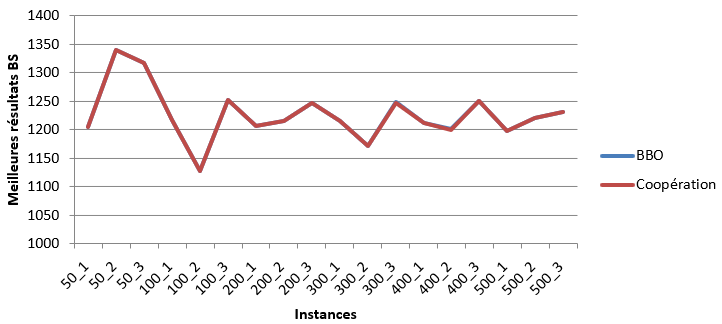
\includegraphics[width=16cm,height=7cm]{Chap5/3.png}
	\caption{Diagrammes d’exécutions de la méthode BBO et la méthode coopérative}
	\label{fig:DEMBBOMC}
\end{figure}

D’après le graphe les deux approches sont similaires. En revanche, en analysant le tableau la meilleure solution (BS) obtenue par la méthode BBO et celle obtenue par l’approche de coopération est pratiquement  la même.

Concernant les moyennes des solutions (AVG), celles obtenues par l’approche coopérative sont de meilleures qualités par rapport à celles obtenues par BBO.
Pour ce qui est le nombre d’évaluation  celui de l’approche coopérative est négligeable comparé à l’autre approche. 

	\item \textbf{Avec l’approche GA}
\begin{table}[H]
	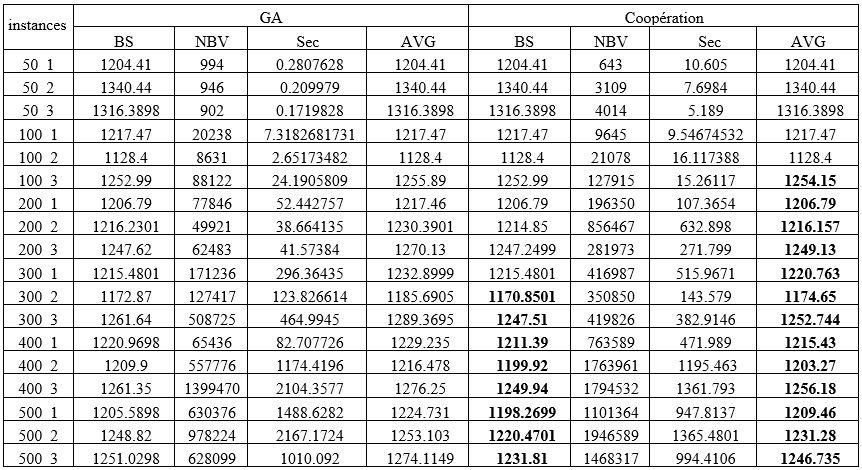
\includegraphics[width=15cm,height=8cm]{Chap5/t4.png}
	\caption{Résultats d’exécutions de GA et la méthode de coopération}
	\label{tab:4}
\end{table}

\begin{figure}[H]
	\centering
	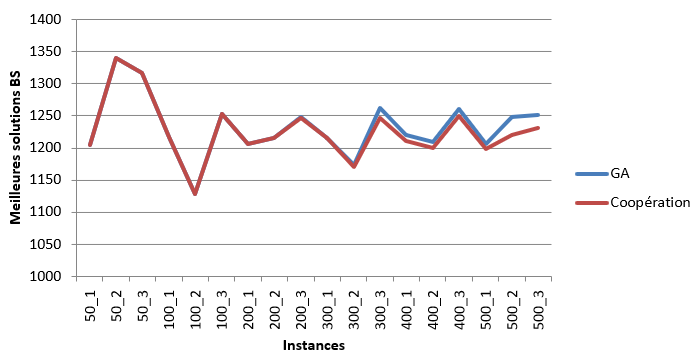
\includegraphics[width=16cm,height=7cm]{Chap5/4.png}
	\caption{Diagrammes d’exécutions de la méthode GA et la méthode coopérative}
	\label{fig:DEMGAMC}
\end{figure}

D’après le graphe \ref{fig:DEMGAMC} et les résultats présentés dans le tableau \ref{tab:4}, les deux approches sont similaires pour les 11 premiers instances la meilleure solution (BS) obtenue par l’approche coopérative  est meilleure que celle obtenue par GA pour les sept  (7) derniers instances. Il faut également noter que la qualité moyenne des solutions (AVG) obtenue par la méthode de coopération est de meilleure qualité que celle obtenue par GA pour toutes les instances du problème. Comparé à GA, le nombre d’évaluation donnée par  l’approche de coopération est relativement faible.

\end{enumerate}


\subsubsection{Comparaison de la méthode coopérative avec les travaux liés au DTP}
Afin de monter l’efficacité et la robustesse de notre approche coopérative, Nous l’avons comparé à deux techniques méta-heuristiques basées sur un essaim dans la littérature, à savoir ACO\_DT [55] et ABC\_DT [54], et une autre méta-heuristique SSGA \cite{sundar2014steady} .

